% Options for packages loaded elsewhere
\PassOptionsToPackage{unicode}{hyperref}
\PassOptionsToPackage{hyphens}{url}
% !TeX program = pdfLaTeX
\documentclass[12pt]{article}
\usepackage{amsmath}
\usepackage{graphicx,psfrag,epsf}
\usepackage{enumerate}
\usepackage[]{natbib}
\usepackage{textcomp}


%\pdfminorversion=4
% NOTE: To produce blinded version, replace "0" with "1" below.
\newcommand{\blind}{0}

% DON'T change margins - should be 1 inch all around.
\addtolength{\oddsidemargin}{-.5in}%
\addtolength{\evensidemargin}{-1in}%
\addtolength{\textwidth}{1in}%
\addtolength{\textheight}{1.7in}%
\addtolength{\topmargin}{-1in}%

%% load any required packages here


% Pandoc syntax highlighting
\usepackage{color}
\usepackage{fancyvrb}
\newcommand{\VerbBar}{|}
\newcommand{\VERB}{\Verb[commandchars=\\\{\}]}
\DefineVerbatimEnvironment{Highlighting}{Verbatim}{commandchars=\\\{\}}
% Add ',fontsize=\small' for more characters per line
\usepackage{framed}
\definecolor{shadecolor}{RGB}{248,248,248}
\newenvironment{Shaded}{\begin{snugshade}}{\end{snugshade}}
\newcommand{\AlertTok}[1]{\textcolor[rgb]{0.94,0.16,0.16}{#1}}
\newcommand{\AnnotationTok}[1]{\textcolor[rgb]{0.56,0.35,0.01}{\textbf{\textit{#1}}}}
\newcommand{\AttributeTok}[1]{\textcolor[rgb]{0.13,0.29,0.53}{#1}}
\newcommand{\BaseNTok}[1]{\textcolor[rgb]{0.00,0.00,0.81}{#1}}
\newcommand{\BuiltInTok}[1]{#1}
\newcommand{\CharTok}[1]{\textcolor[rgb]{0.31,0.60,0.02}{#1}}
\newcommand{\CommentTok}[1]{\textcolor[rgb]{0.56,0.35,0.01}{\textit{#1}}}
\newcommand{\CommentVarTok}[1]{\textcolor[rgb]{0.56,0.35,0.01}{\textbf{\textit{#1}}}}
\newcommand{\ConstantTok}[1]{\textcolor[rgb]{0.56,0.35,0.01}{#1}}
\newcommand{\ControlFlowTok}[1]{\textcolor[rgb]{0.13,0.29,0.53}{\textbf{#1}}}
\newcommand{\DataTypeTok}[1]{\textcolor[rgb]{0.13,0.29,0.53}{#1}}
\newcommand{\DecValTok}[1]{\textcolor[rgb]{0.00,0.00,0.81}{#1}}
\newcommand{\DocumentationTok}[1]{\textcolor[rgb]{0.56,0.35,0.01}{\textbf{\textit{#1}}}}
\newcommand{\ErrorTok}[1]{\textcolor[rgb]{0.64,0.00,0.00}{\textbf{#1}}}
\newcommand{\ExtensionTok}[1]{#1}
\newcommand{\FloatTok}[1]{\textcolor[rgb]{0.00,0.00,0.81}{#1}}
\newcommand{\FunctionTok}[1]{\textcolor[rgb]{0.13,0.29,0.53}{\textbf{#1}}}
\newcommand{\ImportTok}[1]{#1}
\newcommand{\InformationTok}[1]{\textcolor[rgb]{0.56,0.35,0.01}{\textbf{\textit{#1}}}}
\newcommand{\KeywordTok}[1]{\textcolor[rgb]{0.13,0.29,0.53}{\textbf{#1}}}
\newcommand{\NormalTok}[1]{#1}
\newcommand{\OperatorTok}[1]{\textcolor[rgb]{0.81,0.36,0.00}{\textbf{#1}}}
\newcommand{\OtherTok}[1]{\textcolor[rgb]{0.56,0.35,0.01}{#1}}
\newcommand{\PreprocessorTok}[1]{\textcolor[rgb]{0.56,0.35,0.01}{\textit{#1}}}
\newcommand{\RegionMarkerTok}[1]{#1}
\newcommand{\SpecialCharTok}[1]{\textcolor[rgb]{0.81,0.36,0.00}{\textbf{#1}}}
\newcommand{\SpecialStringTok}[1]{\textcolor[rgb]{0.31,0.60,0.02}{#1}}
\newcommand{\StringTok}[1]{\textcolor[rgb]{0.31,0.60,0.02}{#1}}
\newcommand{\VariableTok}[1]{\textcolor[rgb]{0.00,0.00,0.00}{#1}}
\newcommand{\VerbatimStringTok}[1]{\textcolor[rgb]{0.31,0.60,0.02}{#1}}
\newcommand{\WarningTok}[1]{\textcolor[rgb]{0.56,0.35,0.01}{\textbf{\textit{#1}}}}

% tightlist command for lists without linebreak
\providecommand{\tightlist}{%
  \setlength{\itemsep}{0pt}\setlength{\parskip}{0pt}}



\usepackage{booktabs}
\usepackage{longtable}
\usepackage{array}
\usepackage{multirow}
\usepackage{wrapfig}
\usepackage{float}
\usepackage{colortbl}
\usepackage{pdflscape}
\usepackage{tabu}
\usepackage{threeparttable}
\usepackage{threeparttablex}
\usepackage[normalem]{ulem}
\usepackage{makecell}
\usepackage{xcolor}

\IfFileExists{bookmark.sty}{\usepackage{bookmark}}{\usepackage{hyperref}}
\IfFileExists{xurl.sty}{\usepackage{xurl}}{} % add URL line breaks if available
\hypersetup{
  pdftitle={Using Gaussian Mixture Models to Deconstruct Data With Unusual Distributions},
  pdfkeywords={Probability density function; Expectation maximization
algorithm; Multimodality; Pattern recognition},
  hidelinks,
  pdfcreator={LaTeX via pandoc}}



\begin{document}


\def\spacingset#1{\renewcommand{\baselinestretch}%
{#1}\small\normalsize} \spacingset{1}


%%%%%%%%%%%%%%%%%%%%%%%%%%%%%%%%%%%%%%%%%%%%%%%%%%%%%%%%%%%%%%%%%%%%%%%%%%%%%%

\if0\blind
{
  \title{\bf Using Gaussian Mixture Models to Deconstruct Data With
Unusual Distributions}

  \author{
        Cassandra Jin \thanks{The authors gratefully acknowledge
\ldots{}} \\
    Department of Mathematics and Statistics, Amherst College\\
      }
  \maketitle
} \fi

\if1\blind
{
  \bigskip
  \bigskip
  \bigskip
  \begin{center}
    {\LARGE\bf Using Gaussian Mixture Models to Deconstruct Data With
Unusual Distributions}
  \end{center}
  \medskip
} \fi

\bigskip
\begin{abstract}
The text of your abstract. 200 or fewer words. It is intended to provide
an overview of your paper and may be similar to your synopsis. Note that
an abstract can only include one paragraph in this format. You may want
to put your synopsis here as you work to refer to it easily.
\end{abstract}

\noindent%
{\it Keywords:} Probability density function; Expectation maximization
algorithm; Multimodality; Pattern recognition

\vfill

\newpage
\spacingset{1.9} % DON'T change the spacing!

\hypertarget{introduction}{%
\section{Introduction}\label{introduction}}

In the landscape of machine learning, pattern recognition, and data
analysis, the objective and the challenge often lie in capturing
intricate data distributions as effectively as possible. It may be
convenient to assign a single distribution that seems to fit well enough
to a large data set, but it is much more insightful to identify patterns
and clusters within the data. Clustering algorithms such as k-means
clustering provide solutions to finding the patterns within
observations, but such traditional methods still have limitations when
it comes to identifying clusters of different shapes and sizes. For
working with a diverse data set, the Gaussian mixture model (GMM)
employs a combination of multiple Gaussian distributions and, as a
result, excels at capturing the various latent structures within the
data. \citep{kumar2022gaussian}

\begin{figure}
\centering
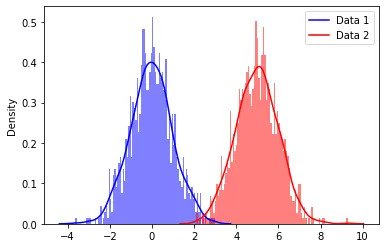
\includegraphics{3.jpg}
\caption{A multimodal distribution, where each peak represents a
different Gaussian distribution or the cluster in the dataset.}
\end{figure}

Like k-means clustering, GMM is a type of machine learning algorithm
used to classify data into different categories based on the probability
distribution. By identifying and merging multiple Gaussian components,
the GMM achieves a parametric probability density function represented
as a weighted sum of Gaussian component densities. The parameters in the
method are estimated from training data using the iterative
expectation-maximization (EM) algorithm, and in maximizing likelihood,
GMM allows a representation of data that goes beyond the limitations of
single-distribution models. The method's ability to model a wide array
of distributions (multimodal, non-Gaussian, etc.) has made GMMs
essential in various domains such as computer vision, speech
recognition, anomaly detection, finance, marketing, and more.

This paper aims to guide readers through the fundamental concepts that
underpin GMMs, offering a comprehensive overview of their mathematical
formulation, the Expectation-Maximization (EM) algorithm employed for
parameter estimation, and the principles that govern their probabilistic
nature. Furthermore, we will explore real-world applications where GMMs
have demonstrated remarkable efficacy, illustrating their relevance and
versatility across diverse domains.

\hypertarget{gaussian-mixture-models-gmms}{%
\section{Gaussian Mixture Models
(GMMs)}\label{gaussian-mixture-models-gmms}}

\label{sec:background}

\hypertarget{the-gaussian-distribution}{%
\subsection{The Gaussian Distribution}\label{the-gaussian-distribution}}

The most basic concept in probability theory and in statistics is the
random variable. A random variable can be understood as a mapping from a
random experiment to a variable, and depending on the nature of the
experiment and the design of the mapping, a random variable can take on
discrete values, continuous values, or a mix of discrete and continuous
values. One possible distribution that the resulting values may follow
is the singular Gaussian distribution, which has probability density
function (PDF)

\begin{equation}
\label{single}
p(x) = \frac{1}{(2\pi)^{1/2} \sigma} exp(-\frac{1}{2}(\frac{x-\mu}{\sigma})^2) \dot{=} N(x; \mu, \sigma^2),
\end{equation}

or \(x \sim N(\mu, \sigma^2)\).

The Gaussian distribution is commonly used in many engineering and
science disciplines due to its highly desirable computational properties
(more detail?), but also from its ability to approximate many naturally
occurring real-world data, due to the law of large numbers.

Expanding this definition, we have that a continuous random variable has
a Gaussian-mixture distribution if its PDF is specified by

\begin{equation}
\label{mix}
p(x) = \sum_{m=1}^M \frac{c_m}{(2\pi)^{1/2} \sigma_m} exp(-\frac{1}{2}(\frac{x-\mu_m}{\sigma_m})^2) = \sum_{m=1}^M c_m N(\mu_m, \sigma_m^2),
\end{equation}

where \(\infty < x < \infty\), \(\sigma_m > 0\), and \(c_m > 0\)
\citep{yu2015gaussian}.

These positive mixture weights sum to 1: \(\sum_{m=1}^M c_m = 1\).

The most obvious property of Gaussian mixture distribution is its
multimodality (\(M>1\) in Equation \ref{mix}), in contrast to the
unimodal property of the Gaussian distribution where \(M=1\). This makes
it possible for GMM to adequately describe many types of physical data
exhibiting multimodality poorly suited for a single Gaussian
distribution.

Based on Equation \ref{mix}, the expectation of a random variable \(x\)
with the mixture Gaussian PDF is \(E(x) = \sum_{m=1}^M c_m \mu_m\). But
unlike a singular, unimodal Gaussian distribution, this simple summary
statistic is not very informative unless all the component means,
\(\mu_m\) for \(m = 1, ..., M\), in the Gaussian-mixture distribution
are close to each other.

Instead, we use the multivariate generalization of the mixture Gaussian
distribution, which has joint PDF

\begin{equation}
\label{joint}
p(x) = \sum_{m=1}^M \frac{c_m}{(2\pi)^{D/2} |\Sigma_m^{1/2}} exp(-\frac{1}{2}(x-\mu_m)^T \Sigma_m^{-1}(x-\mu_m)) = \sum_{m=1}^M c_m N(x; \mu_m, \Sigma_m),
\end{equation}

where \(c_m > 0\).

In using the multivariate mixture Gaussian distribution of Equation
\ref{mix}, if the variable \(x\)'s dimensionality, \(D\), is large
(depends on the context), then the use of full (nondiagonal) covariance
matrices (\(\Sigma_m\)) would involve a large number of parameters. To
reduce the number of parameters, one can instead use diagonal covariance
matrices for \(\Sigma_m\). Alternatively, when \(M\) is large, one can
also constrain all covariance matrices to be the same. The advantage of
using diagonal covariance matrices is significant simplification of
computations needed for the applications of the Gaussian-mixture
distributions.

\hypertarget{parameter-estimation}{%
\subsection{Parameter Estimation}\label{parameter-estimation}}

The Gaussian-mixture distributions discussed above contain a set of
parameters. In the multivariate case of \ref{mix}, the parameter set
consists of \(\Theta = \{c_m, \mu_m, \Sigma_m\}\). The parameter
estimation problem is motivated by wanting to determine the values of
these parameters from data set that we assume to be drawn from the
Gaussian-mixture distribution.

It is common to think of Gaussian mixture modeling and the related
parameter estimation as a missing data problem, and we want to ``learn''
appropriate parameters for the distribution, with the connection to the
data points being represented as their membership in the individual
Gaussian distributions.

Here, we focus on the expectation maximization (EM) algorithm as the
maximum likelihood method of choice for parameter estimation of the
Gaussian-mixture distribution. The EM algorithm is the most popular
technique used to estimate the parameters of a mixture given a fixed
number of mixture components, and it can be used to compute the
parameters of any parametric mixture distribution. The EM algorithm
finds the maximum likelihood of a model through two iterative steps:
expectation or E-step and maximization or M-step. It alternates between
performing an expectation step and a maximization step to achieve
maximum likelihood until a certain stop condition is satisfied or a
specified number of iterations is completed \citep{wan2019novel}.

The EM algorithm is especially fitting to use for GMM, as we can express
the parameters in their closed forms and iterate through the M-step as
follows:

\begin{equation}
\label{c}
c_m^{(j+1)} = \frac{1}{N} \sum_{t=1}^N h_m^{(j)}(t),
\end{equation}

\begin{equation}
\label{mu}
\mu_m^{(j+1)} = \frac{\sum_{t=1}^N h_m^{(j)}(t) x^{(t)}}{\sum_{t=1}^N h_m^{(j)}(t)},
\end{equation}

\begin{equation}
\label{sigma}
\Sigma_m^{(j+1)} = \frac{\sum_{t=1}^N h_m^{(j)}(t) [x^{(t)} - \mu_m^{(j)}][x^{(t)} - \mu_m^{(j)}]^T}{\sum_{t=1}^N h_m^{(j)}(t)},
\end{equation}

The posterior probabilities of these parameters computed from the E-step
are given by

\begin{equation}
\label{posterior}
h_m^{(j)}(t) = \frac{c_m^{(j)} N(x^{(t)}; \mu_m^{(j)}, \Sigma_m^{(j)})}{\sum_{i=1}^n c_i^{(j)} N(x^{(t)}; \mu_i^{(j)}, \Sigma_i^{(j)})}.
\end{equation}

Given the current (denoted by superscript \(j\) above) estimate for the
parameters, the conditional probability for a given observation
\(x^{(t)}\) generated from mixture component \(m\)is determined for each
data sample point at \(t=1, ..., N\), where \(N\) is the sample size.
The parameters then update such that the new component weights
correspond to the average conditional probability, and each component
mean and covariance is the component specific weighted average of the
mean and covariance of the entire sample set.

A particular advantage of the EM algorithm is that each successive
iteration will not decrease the likelihood, a property not shared by
many other maximization techniques. Additionally, the EM algorithm
naturally embeds constraints on the probability vector while avoiding
extra computational costs to check and maintain appropriate values.

\hypertarget{summary}{%
\subsection{Summary}\label{summary}}

Overall, there are three key steps to using Gaussian mixture models for
clustering:

\begin{enumerate}
\def\labelenumi{\arabic{enumi}.}
\item
  Determine a covariance matrix that defines how each Gaussian is
  related to one another. The more similar two Gaussian component
  distributions are, the closer their means will be and vice versa if
  they are far away from each other in terms of similarity. A GMM can
  have a covariance matrix that is diagonal or symmetric (non-diagonal).
\item
  Decide the number of Gaussian models in each group, which dictates how
  many clusters there are.
\item
  Select the hyperparameters that define how the data are optimally
  separated using GMMs.
\end{enumerate}

\hypertarget{connections-and-comparisons-to-other-models}{%
\section{Connections and Comparisons to Other
Models}\label{connections-and-comparisons-to-other-models}}

\label{sec:compare}

Compared with traditional k-means clustering algorithm, GMM has two
primary advantages. Firstly, it takes into account covariance, which
determines the shape of the distribution, so it can fit well when the
distribution of the data presents different shapes. Secondly, while
k-means belongs to hard classification, GMM belongs to soft
classification. This means that k-means clustering outputs a specific
category, whereas GMM outputs the probability of each specific category
the data points belong to, and GMM can therefore estimate the
uncertainty measure of the degree of association between data points and
specific categories \citep{huang2023gaussian}.

As a trade-off of GMMs being more flexible than k-means, they can be
more difficult to train. K-means is typically faster to converge and
more accurate, so it may be preferred in cases where the runtime is an
important consideration or generally when the data set is large and the
clusters are well-separated. On the other hand, GMMs are more accurate
when the data set is small or the clusters are not well-separated.

We know that the EM algorithm enables effective parameter estimation in
probabilistic models with incomplete data. By implementing this
algorithm, Gaussian mixture models can handle missing data, whereas
K-means cannot. This difference makes GMMs more effective in certain
applications where the data contains considerable noise or is not
well-defined \citep{kumar2022gaussian}.

\hypertarget{applications-in-literature}{%
\section{Applications in Literature}\label{applications-in-literature}}

\label{sec:examples}

\begin{itemize}
\tightlist
\item
  Understanding the impact of COVID-19 on energy consumption:
  Researchers used the electricity data set of public buildings in
  Scotland and applied Gaussian Mixture Model (GMM) to explore the
  changes in electricity usage patterns throughout the pandemic, so as
  to understand the long-term impact of COVID-19 on energy consumption
  of public buildings \citep{huang2023gaussian}.
\end{itemize}

\begin{figure}
\centering
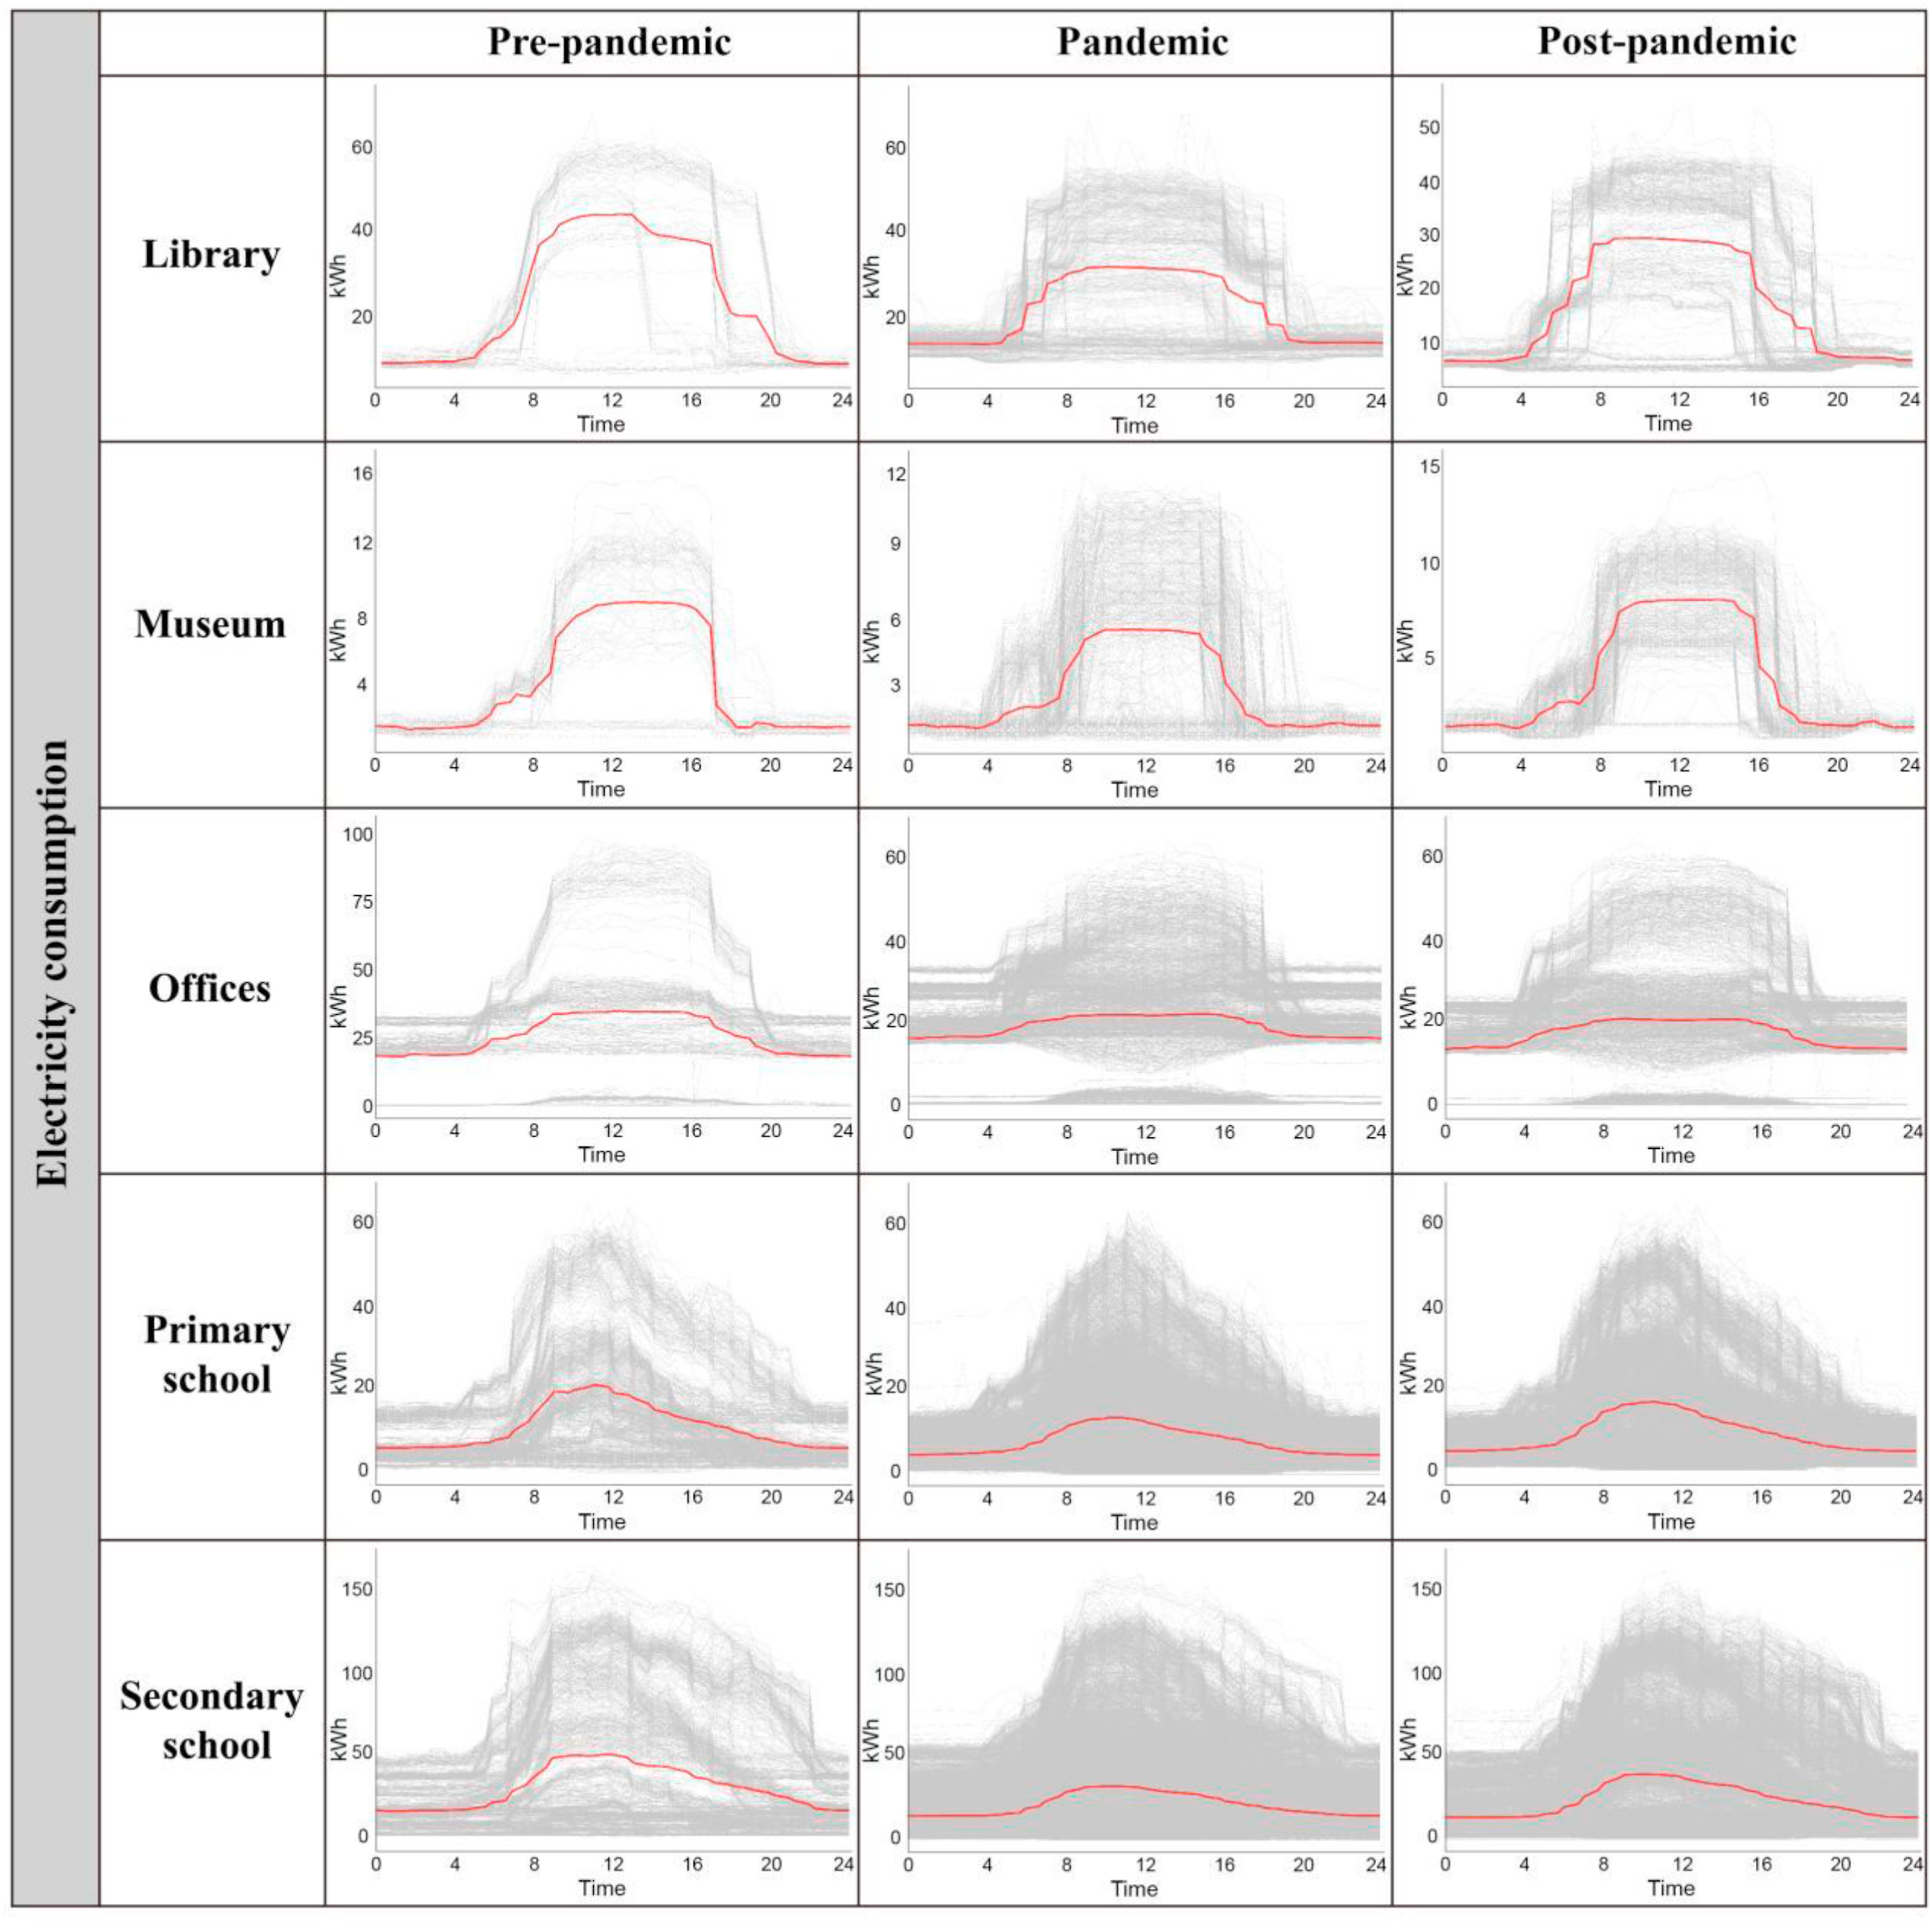
\includegraphics{1.jpg}
\caption{Daily electricity consumption trends of various public
buildings in different periods.}
\end{figure}

\begin{figure}
\centering
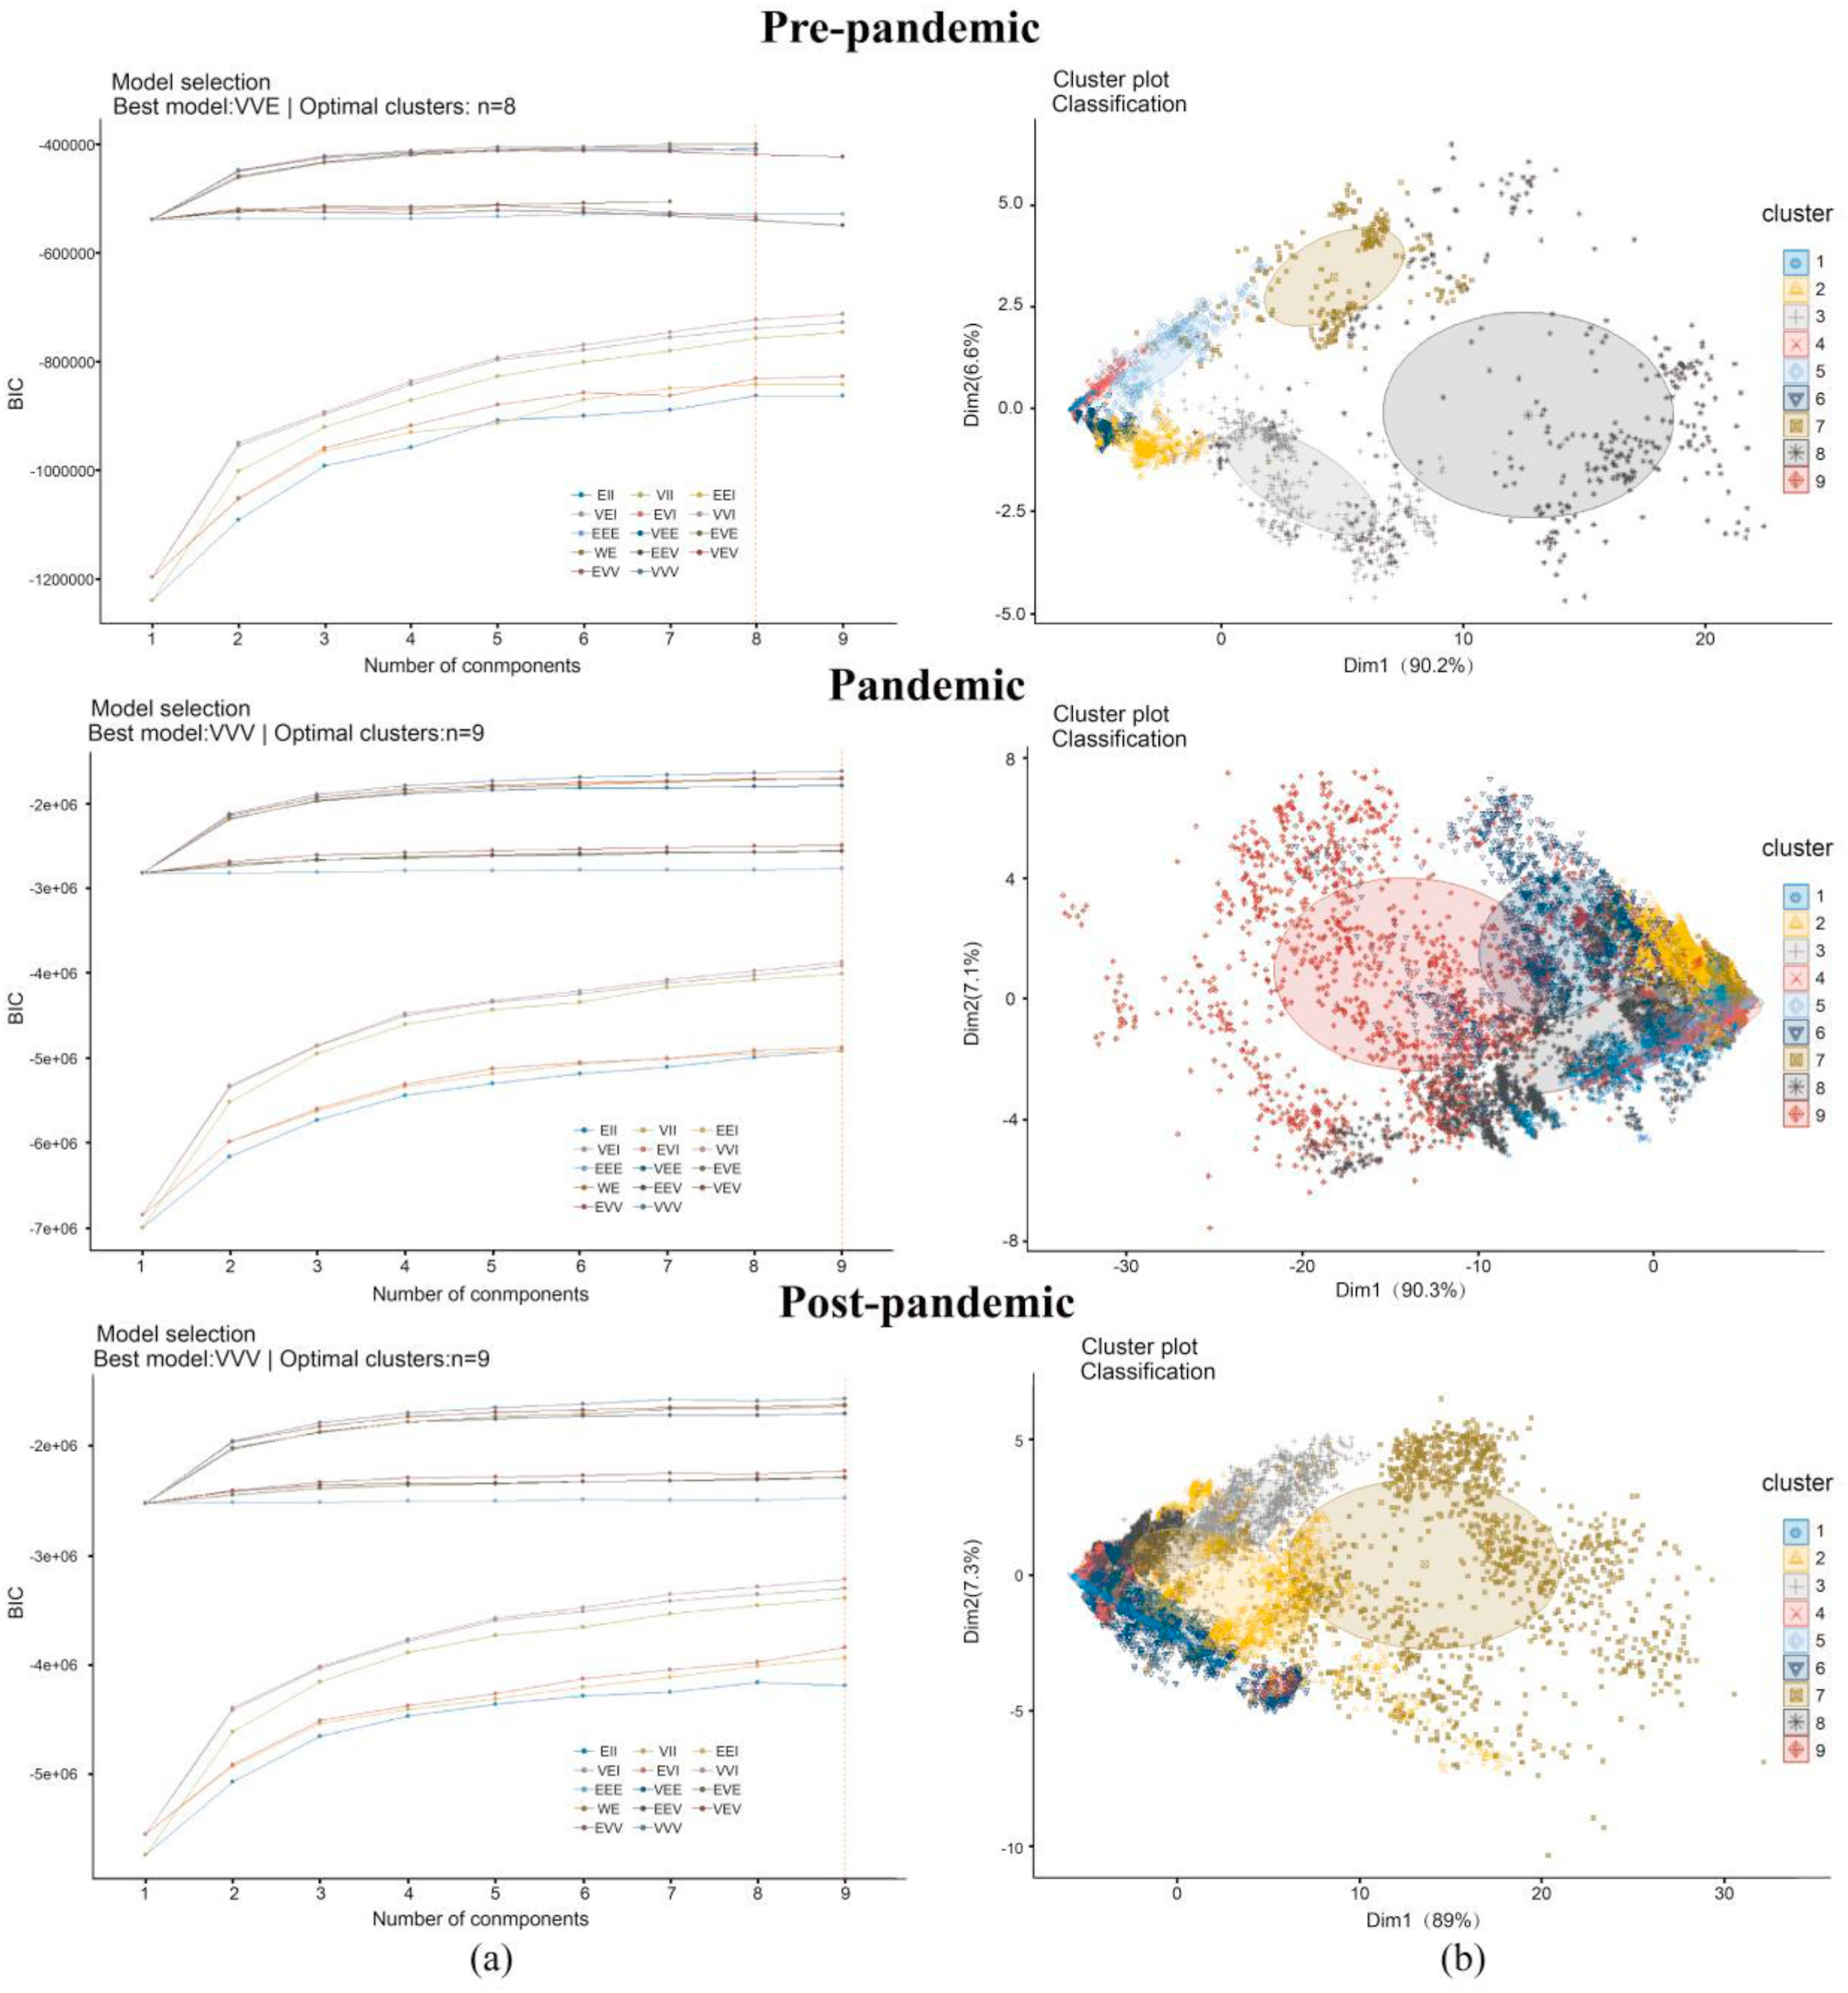
\includegraphics{2.jpg}
\caption{On the right, (b), the visualized Gaussian mixture model for
each condition.}
\end{figure}

\begin{itemize}
\item
  Finding patterns in medical datasets: Medical researchers use GMMs to
  segment images into multiple categories based on their content or to
  find specific patterns in medical datasets. They can determine
  clusters of patients with similar symptoms, identify disease subtypes,
  and even predict outcomes.
\item
  Modeling natural phenomena: GMMs can be used to model natural
  phenomena where it has been found that noise follows Gaussian
  distributions. This model of probabilistic modeling relies on the
  assumption that there exists some underlying continuum of unobserved
  entities or attributes, and that each member is associated with
  measurements taken at equidistant points in multiple observation
  sessions.
\item
  Customer behavior analysis: GMMs can be used for performing customer
  behavior analysis in marketing to make predictions about future
  purchases based on historical data.
\item
  Stock price prediction: In finance, GMMs can be applied to a stock's
  price time series. They can detect changepoints in time series data
  and help find turning points of stock prices or other market movements
  that are otherwise difficult to spot due to volatility and noise.
\item
  Gene expression data analysis: GMMs can be used to detect
  differentially expressed genes between two conditions and to identify
  which genes might contribute toward a certain phenotype or disease
  state.
\end{itemize}

\hypertarget{implementation-in-r}{%
\section{Implementation in R}\label{implementation-in-r}}

\hypertarget{single-component-without-missingness}{%
\subsection{Single Component Without
Missingness}\label{single-component-without-missingness}}

For \(n\) observations on \(d\) dimensional data, we can introduce a
fraction of missing values \(m\) completely at random by setting
elements of the data set to NA.

Here, \(n = 1e3\) observations are simulated from a single \(k = 1\)
bivariate normal distribution \(d = 2\) without missingness (miss = 0,
by default). The mean is \(\mu = (2, 2)\), and the covariance is an
exchangeable correlation structure with off-diagonal \(\rho = 0.5\).

\begin{Shaded}
\begin{Highlighting}[]
\FunctionTok{set.seed}\NormalTok{(}\DecValTok{495}\NormalTok{)}
\NormalTok{sigma }\OtherTok{\textless{}{-}} \FunctionTok{matrix}\NormalTok{(}\FunctionTok{c}\NormalTok{(}\DecValTok{1}\NormalTok{, }\FloatTok{0.5}\NormalTok{, }\FloatTok{0.5}\NormalTok{, }\DecValTok{1}\NormalTok{), }\AttributeTok{nrow =} \DecValTok{2}\NormalTok{)}
\NormalTok{data }\OtherTok{=} \FunctionTok{rGMM}\NormalTok{(}\AttributeTok{n =} \FloatTok{1e3}\NormalTok{, }\AttributeTok{d =} \DecValTok{2}\NormalTok{, }\AttributeTok{k =} \DecValTok{1}\NormalTok{, }\AttributeTok{means =} \FunctionTok{c}\NormalTok{(}\DecValTok{2}\NormalTok{, }\DecValTok{2}\NormalTok{), }\AttributeTok{covs =}\NormalTok{ sigma)}
\NormalTok{fit }\OtherTok{\textless{}{-}} \FunctionTok{FitGMM}\NormalTok{(data, }\AttributeTok{k =} \DecValTok{1}\NormalTok{)}
\FunctionTok{show}\NormalTok{(fit)}
\end{Highlighting}
\end{Shaded}

\begin{verbatim}
## Multivariate Normal Model. 
## 
## Estimated mean:
##   y1   y2 
## 2.01 2.00 
## 
## Estimated covariance:
##       y1    y2
## y1 0.963 0.475
## y2 0.475 1.020
## 
## Final Objective:
## [1] -1720
\end{verbatim}

\hypertarget{single-component-with-missingness}{%
\subsection{Single Component With
Missingness}\label{single-component-with-missingness}}

\(n = 1e3\) observations are simulated from a single \(k = 1\)
trivariate normal distribution \(d = 3\) with 20\% missingness (miss =
0.2). The mean defaults to the zero vector, and the covariance to the
identity matrix.

\begin{Shaded}
\begin{Highlighting}[]
\FunctionTok{set.seed}\NormalTok{(}\DecValTok{495}\NormalTok{)}
\NormalTok{sigma }\OtherTok{\textless{}{-}} \FunctionTok{matrix}\NormalTok{(}\FunctionTok{c}\NormalTok{(}\DecValTok{1}\NormalTok{, }\FloatTok{0.5}\NormalTok{, }\FloatTok{0.5}\NormalTok{, }\DecValTok{1}\NormalTok{), }\AttributeTok{nrow =} \DecValTok{2}\NormalTok{)}
\NormalTok{data }\OtherTok{=} \FunctionTok{rGMM}\NormalTok{(}\AttributeTok{n =} \FloatTok{1e3}\NormalTok{, }\AttributeTok{d =} \DecValTok{3}\NormalTok{, }\AttributeTok{k =} \DecValTok{1}\NormalTok{, }\AttributeTok{miss =} \FloatTok{0.2}\NormalTok{)}
\NormalTok{fit }\OtherTok{\textless{}{-}} \FunctionTok{FitGMM}\NormalTok{(data, }\AttributeTok{k =} \DecValTok{1}\NormalTok{)}
\end{Highlighting}
\end{Shaded}

\begin{verbatim}
## Objective increment:  2.76 
## Objective increment:  0.135 
## Objective increment:  0.00904 
## Objective increment:  0.000855 
## Objective increment:  0.000101 
## Objective increment:  1.33e-05 
## Objective increment:  1.82e-06 
## Objective increment:  2.55e-07 
## 7 update(s) performed before reaching tolerance limit.
\end{verbatim}

\begin{Shaded}
\begin{Highlighting}[]
\FunctionTok{show}\NormalTok{(fit)}
\end{Highlighting}
\end{Shaded}

\begin{verbatim}
## Multivariate Normal Model. 
## 
## Estimated mean:
##      y1      y2      y3 
## 0.01740 0.02460 0.00185 
## 
## Estimated covariance:
##         y1      y2     y3
## y1  0.9700 -0.0303 0.0227
## y2 -0.0303  1.0400 0.0363
## y3  0.0227  0.0363 1.0700
## 
## Final Objective:
## [1] -3040
\end{verbatim}

\hypertarget{clustering-quality}{%
\subsection{Clustering Quality}\label{clustering-quality}}

The function \texttt{ClustQual} provides several metrics for internally
assessing the quality of cluster assignments from a fitted GMM. The
output is a list containing the following metrics:

\begin{itemize}
\item
  BIC (Bayesian information criterion): a penalized version of the
  negative log likelihood. A lower value indicates better clustering
  quality.
\item
  CHI (Calinski-Harabaz index): a ratio of the between-cluster to
  within-cluster variation. A higher value indicates better clustering
  quality.
\item
  DBI (Davies-Bouldin index): an average of similarities across
  clusters. A lower value indicates better clustering quality.
\item
  SIL: average silhouette width, a measure of how well an observation
  matches its assigned cluster. A higher value indicates better
  clustering quality.
\end{itemize}

\begin{Shaded}
\begin{Highlighting}[]
\FunctionTok{set.seed}\NormalTok{(}\DecValTok{495}\NormalTok{)}
\NormalTok{mu }\OtherTok{\textless{}{-}} \FunctionTok{list}\NormalTok{(}
  \FunctionTok{c}\NormalTok{(}\DecValTok{2}\NormalTok{, }\DecValTok{2}\NormalTok{),}
  \FunctionTok{c}\NormalTok{(}\DecValTok{2}\NormalTok{, }\SpecialCharTok{{-}}\DecValTok{2}\NormalTok{),}
  \FunctionTok{c}\NormalTok{(}\SpecialCharTok{{-}}\DecValTok{2}\NormalTok{, }\DecValTok{2}\NormalTok{),}
  \FunctionTok{c}\NormalTok{(}\SpecialCharTok{{-}}\DecValTok{2}\NormalTok{, }\SpecialCharTok{{-}}\DecValTok{2}\NormalTok{)}
\NormalTok{)}
\NormalTok{sigma }\OtherTok{\textless{}{-}} \FloatTok{0.5} \SpecialCharTok{*} \FunctionTok{diag}\NormalTok{(}\DecValTok{2}\NormalTok{)}
\NormalTok{data }\OtherTok{=} \FunctionTok{rGMM}\NormalTok{(}\AttributeTok{n =} \DecValTok{100}\NormalTok{, }\AttributeTok{d =} \DecValTok{2}\NormalTok{, }\AttributeTok{k =} \DecValTok{4}\NormalTok{, }\AttributeTok{means =}\NormalTok{ mu, }\AttributeTok{covs =}\NormalTok{ sigma)}
\NormalTok{fit }\OtherTok{\textless{}{-}} \FunctionTok{FitGMM}\NormalTok{(data, }\AttributeTok{k =} \DecValTok{4}\NormalTok{, }\AttributeTok{maxit =} \DecValTok{100}\NormalTok{, }\AttributeTok{eps =} \FloatTok{1e{-}8}\NormalTok{, }\AttributeTok{report =}\NormalTok{ F)}

\CommentTok{\#quality metrics}
\NormalTok{clust\_qual }\OtherTok{=} \FunctionTok{ClustQual}\NormalTok{(fit)}
\FunctionTok{cat}\NormalTok{(}\StringTok{"BIC:}\SpecialCharTok{\textbackslash{}n}\StringTok{"}\NormalTok{)}
\end{Highlighting}
\end{Shaded}

\begin{verbatim}
## BIC:
\end{verbatim}

\begin{Shaded}
\begin{Highlighting}[]
\NormalTok{clust\_qual}\SpecialCharTok{$}\NormalTok{BIC}
\end{Highlighting}
\end{Shaded}

\begin{verbatim}
## [1] 221.9521
\end{verbatim}

\begin{Shaded}
\begin{Highlighting}[]
\FunctionTok{cat}\NormalTok{(}\StringTok{"}\SpecialCharTok{\textbackslash{}n}\StringTok{CHI:}\SpecialCharTok{\textbackslash{}n}\StringTok{"}\NormalTok{)}
\end{Highlighting}
\end{Shaded}

\begin{verbatim}
## 
## CHI:
\end{verbatim}

\begin{Shaded}
\begin{Highlighting}[]
\NormalTok{clust\_qual}\SpecialCharTok{$}\NormalTok{CHI}
\end{Highlighting}
\end{Shaded}

\begin{verbatim}
## [1] 10.17547
\end{verbatim}

\begin{Shaded}
\begin{Highlighting}[]
\FunctionTok{cat}\NormalTok{(}\StringTok{"}\SpecialCharTok{\textbackslash{}n}\StringTok{DBI:}\SpecialCharTok{\textbackslash{}n}\StringTok{"}\NormalTok{)}
\end{Highlighting}
\end{Shaded}

\begin{verbatim}
## 
## DBI:
\end{verbatim}

\begin{Shaded}
\begin{Highlighting}[]
\NormalTok{clust\_qual}\SpecialCharTok{$}\NormalTok{DBI}
\end{Highlighting}
\end{Shaded}

\begin{verbatim}
## [1] 0.470887
\end{verbatim}

\begin{Shaded}
\begin{Highlighting}[]
\FunctionTok{cat}\NormalTok{(}\StringTok{"}\SpecialCharTok{\textbackslash{}n}\StringTok{SIL:}\SpecialCharTok{\textbackslash{}n}\StringTok{"}\NormalTok{)}
\end{Highlighting}
\end{Shaded}

\begin{verbatim}
## 
## SIL:
\end{verbatim}

\begin{Shaded}
\begin{Highlighting}[]
\NormalTok{clust\_qual}\SpecialCharTok{$}\NormalTok{SIL}
\end{Highlighting}
\end{Shaded}

\begin{verbatim}
## [1] 0.6393902
\end{verbatim}

\hypertarget{choosing-the-number-of-clusters}{%
\subsection{Choosing the Number of
Clusters}\label{choosing-the-number-of-clusters}}

The function \texttt{ChooseK} provides guidance on the number of
clusters present in data where the number of clusters \(k\) is unknown.
The inputs include the data matrix, the minimum number of clusters to
assess k0, the maximum number of clusters to assess k1, and the number
of bootstrap replicates at each cluster number boot. For each cluster
number k from k0 to k1, bootstrapped data sets are generated. A GMM with
\(k\) components is fit, and the quality metrics are calculated. The
bootstrap replicates are summarized by their mean and standard error
(SE). For each quality metric, the output contains the cluster number
k\_opt that provides the optimal quality and the smallest cluster number
whose quality is within 1 SE of the optimum k\_1se.

\begin{Shaded}
\begin{Highlighting}[]
\NormalTok{choose\_k }\OtherTok{\textless{}{-}} \FunctionTok{ChooseK}\NormalTok{(data, }\AttributeTok{k0 =} \DecValTok{2}\NormalTok{, }\AttributeTok{k1 =} \DecValTok{6}\NormalTok{, }\AttributeTok{boot =} \DecValTok{10}\NormalTok{)}
\end{Highlighting}
\end{Shaded}

\begin{verbatim}
## Cluster size 2 complete. 11 fit(s) succeeded.
## Cluster size 3 complete. 11 fit(s) succeeded.
## Cluster size 4 complete. 11 fit(s) succeeded.
## Cluster size 5 complete. 11 fit(s) succeeded.
## Cluster size 6 complete. 10 fit(s) succeeded.
\end{verbatim}

\begin{Shaded}
\begin{Highlighting}[]
\FunctionTok{cat}\NormalTok{(}\StringTok{"}\SpecialCharTok{\textbackslash{}n}\StringTok{Cluster number choices:}\SpecialCharTok{\textbackslash{}n}\StringTok{"}\NormalTok{)}
\end{Highlighting}
\end{Shaded}

\begin{verbatim}
## 
## Cluster number choices:
\end{verbatim}

\begin{Shaded}
\begin{Highlighting}[]
\NormalTok{choose\_k}\SpecialCharTok{$}\NormalTok{Choices}
\end{Highlighting}
\end{Shaded}

\begin{verbatim}
##   Metric k_opt  Metric_opt k_1se  Metric_1se
## 1    BIC     6 151.3227726     5 157.3881681
## 2    CHI     6  15.7701771     6  15.7701771
## 3    DBI     4   0.4754451     4   0.4754451
## 4    SIL     4   0.6443205     4   0.6443205
\end{verbatim}

\begin{Shaded}
\begin{Highlighting}[]
\FunctionTok{cat}\NormalTok{(}\StringTok{"}\SpecialCharTok{\textbackslash{}n}\StringTok{All results:}\SpecialCharTok{\textbackslash{}n}\StringTok{"}\NormalTok{)}
\end{Highlighting}
\end{Shaded}

\begin{verbatim}
## 
## All results:
\end{verbatim}

\begin{Shaded}
\begin{Highlighting}[]
\FunctionTok{head}\NormalTok{(choose\_k}\SpecialCharTok{$}\NormalTok{Results)}
\end{Highlighting}
\end{Shaded}

\begin{verbatim}
##   Clusters Fits Metric        Mean          SE
## 1        2   11    BIC 331.1585430  7.83821234
## 2        2   11    CHI   1.9099133  0.18458241
## 3        2   11    DBI   0.9500322  0.05248028
## 4        2   11    SIL   0.4765720  0.01810555
## 5        3   11    BIC 273.7737692 16.45488885
## 6        3   11    CHI   3.9120636  0.26041417
\end{verbatim}

\hypertarget{application-to-data}{%
\section{Application to Data}\label{application-to-data}}

\bibliographystyle{plainnat}
\renewcommand\refname{Conclusion}
\bibliography{bibliography.bib}



\end{document}
